\section{Implications}

\begin{figure}[ht]
\centering
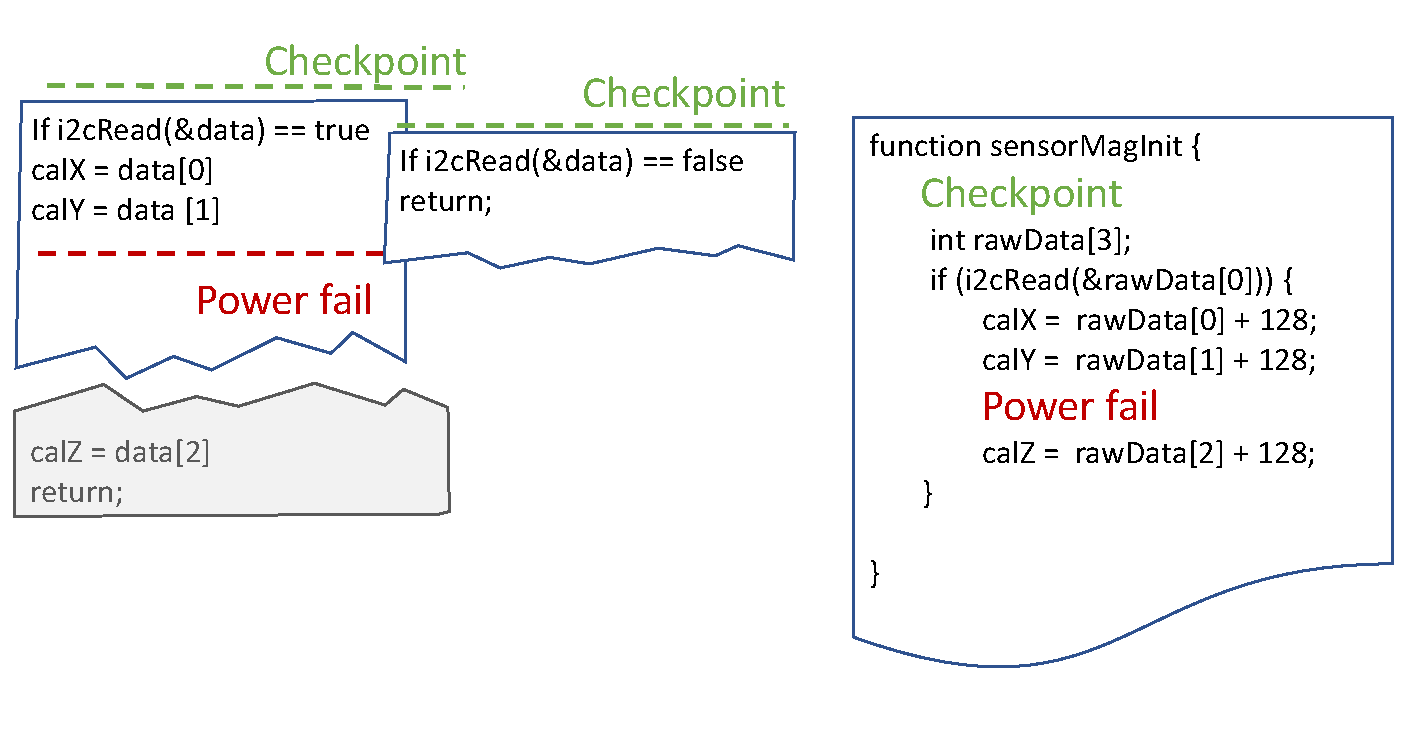
\includegraphics[width=1\columnwidth]{maginit_bug.pdf}
\caption{Bug in magnetometer initialization. Power failing while updating the calibration fields can cause the calibration data to become inconsistent, corrupting any future magnetometer reads that use the calibration.}
\label{fig:mag}
\end{figure}

\begin{figure}[ht]
\centering
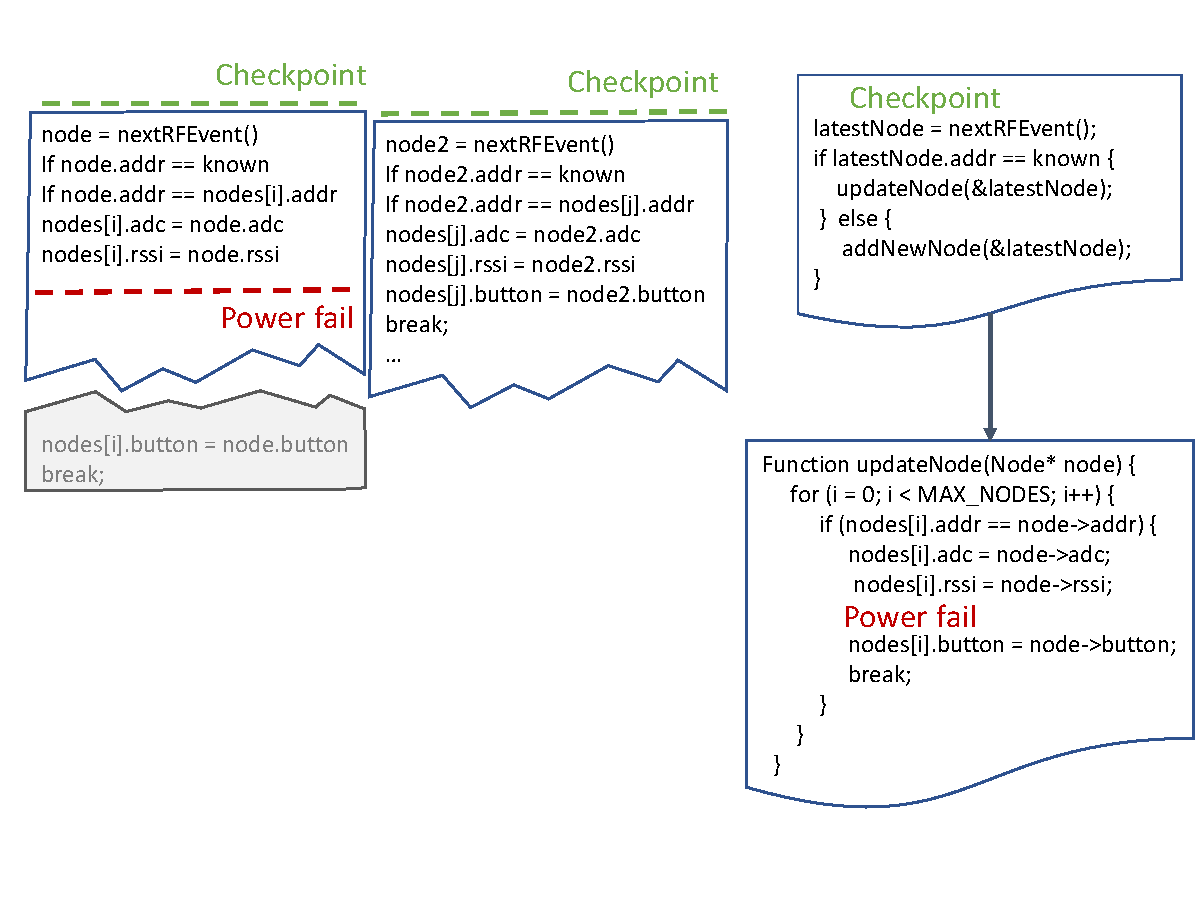
\includegraphics[width=1\columnwidth]{wsn_concentrator_bug.pdf}
\caption{Bug in WSN concentrator. Power failing while updating the node structure can cause the node list to become inconsistent, corrupting the payload ("button" field) or using out-of-date timing information}
\label{fig:wsn}
\end{figure}

\begin{figure}[ht]
\centering
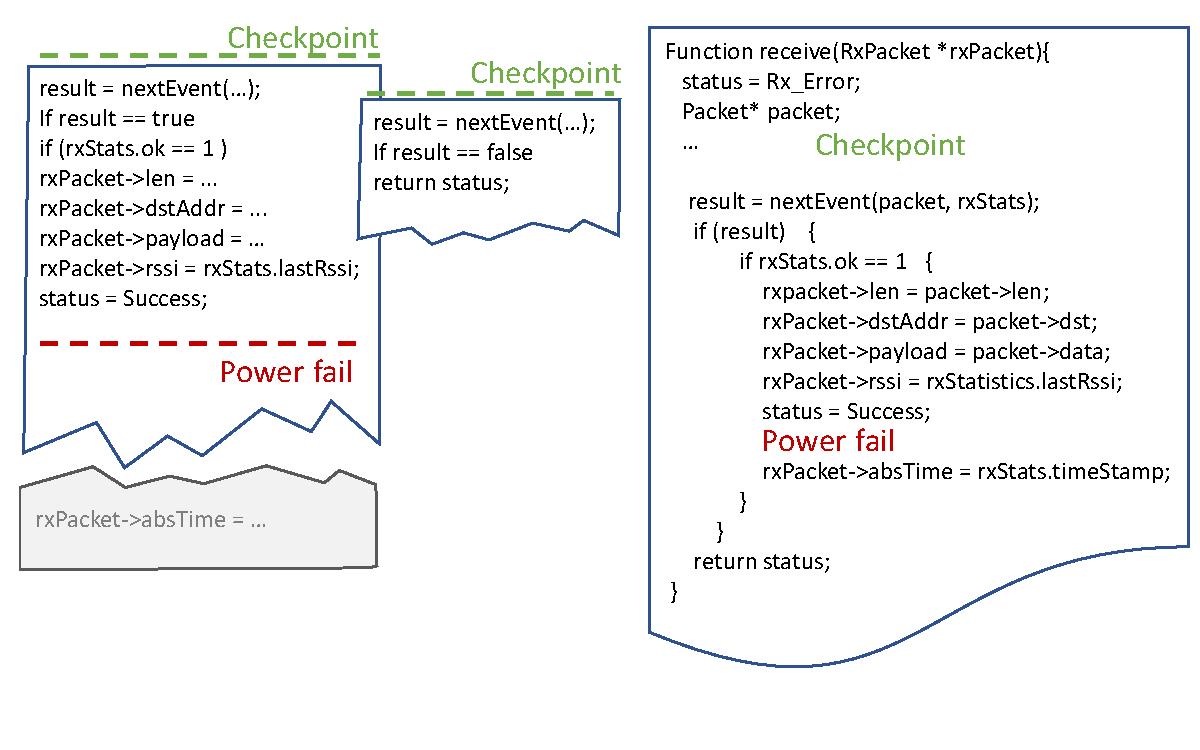
\includegraphics[width=1\columnwidth]{easylinkrx_bug.pdf}
\caption{Bug in RF EasyLink Receiver. Power failing before returning a correctly read packet can cause the status field to be set to success, even if the next event fails. The function will return an incorrect status value, potentially crashing the larger application.}
\label{fig:rf}
\end{figure}